% \documentclass{sig-alternate}
\documentclass[conference]{IEEEtran}


%\renewcommand\IEEEkeywordsname{Some words}

\usepackage{cite}
\usepackage{url}
\usepackage{color}
\usepackage{tikz}
\usepackage{balance}
\usepackage{caption}
\usepackage{soul} % Used for highlighting % \hl{this is some highlighted text}
\usepackage{times} % Used for formatting formatting url footnotes
\urlstyle{same} % Used for formatting formatting url footnotes

%%% Messes with the alignment of the table headers
% \RequirePackage[singlelinecheck=off]{caption}
%\captionsetup{justification=centering}

\newcommand{\todo}[1]{\textcolor{cyan}{\textbf{[#1]}}}
\newcommand{\Sam}[1]{\textcolor{green}{{\it [Sam says: #1]}}}
\newcommand{\dan}[1]{\textcolor{blue}{{\it [Dan says: #1]}}}
\newcommand{\Mehdi}[1]{\textcolor{red}{{\it [Mehdi says: #1]}}}


% Define flow chart styles
\tikzstyle{decision} = [diamond, draw, fill=blue!20,
    text width=15em, text badly centered, node distance=3cm, inner sep=0pt]
\tikzstyle{block} = [rectangle, draw, fill=blue!20,
    text width=15em, text centered, rounded corners, minimum height=4em]
\tikzstyle{line} = [draw, -latex']

\usetikzlibrary{shapes,arrows, positioning} % Needed for analysis diagram


%\conferenceinfo{MSR}{'15, May 16 ? June 1, 2014, Florence, Italy}
%\CopyrightYear{2015}
%%\crdata{978-1-4503-2863-0/14/05}
%\crdata{xxxxxxxxxx}


\clubpenalty = 10000
\widowpenalty = 10000
\displaywidowpenalty = 10000

\usepackage{flushend} 
\begin{document}

%\conferenceinfo{MSR}{'15 Florence, Italy}


% A Dataset of Open Source Android Applications

\title{A Dataset of Open-Source Android Applications}

\author{\IEEEauthorblockN{Daniel E. Krutz, Mehdi Mirakhorli, Samuel~A.~Malachowsky, Andres Ruiz, \\Jacob~Peterson, Andrew~Filipski, and Jared Smith}
\IEEEauthorblockA{
Rochester Institute of Technology,
Rochester, NY, USA\\
\{dxkvse, mxmvse, samvse, ajr2546, jrp9988, abf1932, jps6773\}@rit.edu}


}
 % Must not be a space above this

\maketitle
\begin{abstract}

%In this paper, we present the results of static analysis when performed on a large dataset of Android apps from F-Droid, an open-source Android app repo.


Android has grown to be the world's most popular mobile platform with~\emph{apps} that are capable of doing everything from checking sports scores to purchasing stocks. In order to assist researchers and developers in better understanding the development process as well as the current state of the apps themselves, we present a large dataset of analyzed open-source Android applications and provide a brief analysis of the data, demonstrating potential usefulness. This dataset contains 1,179 applications, including 4,416 different versions of these apps and 435,680 total commits. Furthermore, for each app we include the analytical results obtained from several static analysis tools including Androguard, Sonar, and Stowaway.

In order to better support the community in conducting research on the security characteristics of the apps, our large analytical dataset comes with the detailed information including various versions of AndroidManifest.xml files and synthesized information such as permissions, intents, and minimum SDK. We collected 13,036 commits of the manifest files and recorded over 69,707 total permissions used.
The results and a brief set of analytics are presented on our website: http://androsec.rit.edu.
\end{abstract}


%%% Are these good keywords???
\begin{keywords}
%Broad band networks, quality of service, WDM.
Open-source dataset, Android development, Software Engineering

\end{keywords} 


%\begin{IEEEkeywords}
%This, that.
%\end{IEEEkeywords}

% \begin{center} \bfseries EDICS Category: 3-BBND \end{center}

%\begin{IEEEkeywords}
%Computer Society, IEEEtran, journal, \LaTeX, paper, template.
%\end{IEEEkeywords}

% Update these ?
%\category{D.2.3}{Software Engineering}{Coding Tools and Techniques}
%\category{D.2.13}{Software Engineering}{Reusable Software}
%\terms{Maintaining software, Reusability, Software Evolution}
%\keywords{Mobile Application Development, Android, Software Engineering}
%% \todo{update keywords}

\section{Introduction}



\begin{table*}
\centering
\makebox[0pt][c]{\parbox{0.95\textwidth}{%
    \begin{minipage}[b]{0.32\hsize}\centering
    \begin{center}
        \caption{Data Overview}
        \label{table:dataoverview}
        \begin{tabular}{| r |l|r | } \hline
        \bfseries  & \bfseries Value & \bfseries Count  \\ \hline %\hline
          \bfseries Totals & \bfseries Apps & 1,179    \\ \cline{2-3}
        & \bfseries Versions & 4,416   \\ \cline{2-3}
        & \bfseries Commiters & 4,535  \\ \cline{2-3}
        & \bfseries Committs & 435,680  \\ \cline{2-3}
        %& \bfseries x & x  \\ \cline{2-3}
        %& \bfseries Avg. & \bfseries \\ \cline{2-3}
         \hline %\hline
          \bfseries Largest & \bfseries Versions & 48     \\ \cline{2-3}
        &   \bfseries Committers & 202     \\ \cline{2-3}
        & \bfseries Commits & 65,110  \\ \cline{2-3}
        %& \bfseries x & x   \\ \cline{2-3}
        %& \bfseries Avg. & \bfseries x  \\ \cline{2-3}
         \hline
        \end{tabular}
        \end{center}
            \end{minipage}
            \hfill
            \begin{minipage}[b]{0.32\hsize}\centering
                \begin{center}
        \caption{Version Counts}
        \label{table:VersionCount}
        \begin{tabular}{ | l | r | }
          \hline
          \bfseries Min Versions & \bfseries Count \\ \hline

        	3 &	466 \\ \hline
        	5 &	258  \\ \hline
        	10 &	97 \\ \hline
        	15 &	54 \\ \hline
        	20 &	26 \\ \hline
        	25 &	16 \\ \hline
        	30+ & 12 \\ \hline

         \end{tabular}
        \end{center}

    \end{minipage}
    \hfill
    \begin{minipage}[b]{0.32\hsize}\centering
       \caption{Commit Keywords}
        \label{table:KeywordCount}
       \begin{tabular}{ | l | r | }
              \hline
              \bfseries Keyword & \bfseries Version Count \\ \hline
              Fix & 81,558 \\ \hline
              Bug & 21,380 \\ \hline
              Version & 14,031 \\ \hline
              Hack & 1,707 \\ \hline
              Performance & 809 \\ \hline
              Permission & 700 \\ \hline
              Failure & 512  \\ \hline
              Security & 148 \\ \hline

              % Vulnerability & 1  \\ \hline

            \end{tabular}

    \end{minipage}%
}}
\end{table*}






\begin{table*}
\centering
\makebox[0pt][c]{\parbox{0.86\textwidth}{%
    \begin{minipage}[b]{0.32\hsize}\centering
    \begin{center}



\caption{Committer Count}
\label{table:CountsbyCommits}
\begin{tabular}{ |l|l|r|r|r |}
\hline
& & \multicolumn{3}{| c | }{\bfseries  Min Commit Count} \\ \hline
  & & \bfseries 10 & \bfseries 25 & \bfseries 50 \\ \hline %\hline

          \bfseries Count of & \bfseries Apps    & 118 & 53 &  23   \\ \cline{2-5}
 &   \bfseries  Categories    & 13 & 13 &  11 \\ \hline %\hline

     \bfseries Avg & \bfseries Commiter Count    & 35 & 60 &  94   \\ \cline{2-5}
 &  \bfseries  Commit Count   & 2,841 & 5,233 &  9,240 \\ \hline

%     \bfseries Max & \bfseries Commiter Count    & x &  &  x  \\ \cline{2-5}
%&    \bfseries Commit Count    & x & x &  x \\  \hline

        \end{tabular}
        \end{center}
            \end{minipage}
            \hfill
            \begin{minipage}[b]{0.32\hsize}\centering
              %  \begin{center}
            \caption{Permission Counts}
            \label{table:PermissionCounts}
                \begin{tabular}{ | l | r | }
          \hline
          \bfseries Permission & \bfseries Count \\ \hline

                INTERNET & 9,049 \\ \hline
                WRITE\_EXTERNAL\_STORAGE &6,518 \\ \hline
                ACCESS\_NETWORK\_STATE & 5,778 \\ \hline
                WAKE\_LOCK &3,886 \\ \hline
                RECEIVE\_BOOT\_COMPLETED & 3,402 \\ \hline

         \end{tabular}
      %  \end{center}

    \end{minipage}

}}
\end{table*}





% What is the problem we are trying to solve.
Android has become an extremely popular mobile platform, and Android apps are not immune to the problems which have hindered traditional software --- especially security vulnerabilities, high maintenance costs, and bugs. Understanding how software is created and maintained is paramount in determining how to produce it faster, cheaper, and of higher quality. One way to gain valuable insight into the development process is to examine existing projects: source code, how the app has evolved over time, and attributes such as its security, defects, and size. App source code may be analyzed using static analysis tools, providing data about the software's security risk level, possible defects, or even lack of adherence to coding standards. Studying version control history can provide information about how the app was created --- especially through the examination of commit messages, who made the commit, and when it was made.


We have created a dataset of 1,179 open-source Android apps with 435,680 version control commits through the mining of F-Droid\footnote{https://f-droid.org}, a repository of Android apps of various sizes and categories. In this paper we discuss (i) the data collection and analysis process, (ii) web portal developed to share the data as well as analytical results in an easy to use manner, and (iii) different characteristics and attributes of this dataset. Our goal is to create a publicly available dataset which researchers can utilize to conduct more comprehensive experiments on Android app development.

\section{Related Work}
\label{sec: relatedworks}

While we are unaware of any projects which have gathered such a substantial amount of Android data, performed various types of static analysis upon it, and made is as publicly available as we did, there are several existing commercial websites which do provide metics about Android applications. Appannie\footnote{http://www.appannie.com}, AppBrain\footnote{http://www.appbrain.com}, and AppZoom\footnote{http://www.appszoom.com} contain analytical and statistical information about hundreds of thousands of Android apps in a  robust and easy to use online format. They do not appear to make their data fully transparent or examine the version histories as we have done.

A large number of previous works have analyzed version control systems for various software engineering purposes. Eyolfson et al.\cite{Eyolfson:2011:TDD:1985441.1985464} examined the effects that developer experience, and date and time of commit had on the bugginess of an application. Buse and Weimer\cite{Buse:2010:ADP:1858996.1859005} used commit messages to automatically document program changes. While we do not perform any data analysis in this paper, the previous use of version control information for software engineering research demonstrates the importance and relevance of our dataset.



\section{Dataset Construction}
\label{sec: datasetconstruction}

% Add short introduction here

Our dataset was built in two primary phases: the data collection process which included gathering source code and version control information from the F-Droid repository, and an analysis using several static analysis tools. An overview of the process is shown in Figure~\ref{fig:ap}.


\begin{figure}[tbph]
\centering
\vspace{-0.2cm}
% 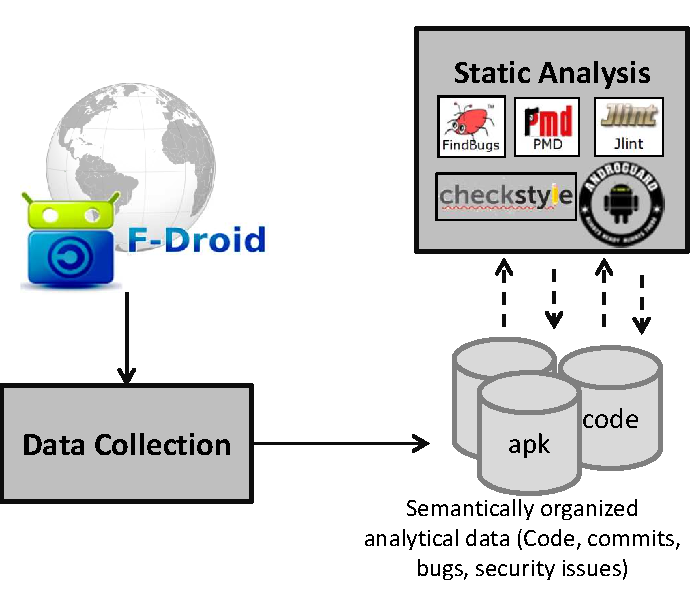
\includegraphics[width=0.9\linewidth]{./images/img}
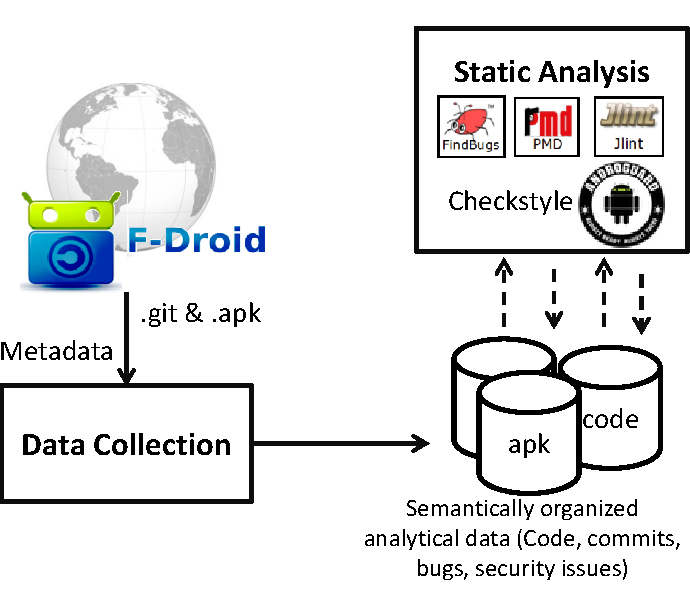
\includegraphics[scale=.6]{./images/collectionprocess.pdf}
\caption{Collection \& Analysis Process}
\vspace{-0.2cm}
\label{fig:ap}
\end{figure}


\subsection{Collection Process}

For the first phase we built a scraper tool to collect data from the F-Droid repository, extracting information from each app such as meta-data (name, description, and version), the source code of each major version, and its most recent apk (Android application) file.  Additionally, we collected version control information such as the committer user name, commit time, and commit messages, ensuring all data was tagged with the version number to allow analysis over time.

%These security settings are stored in the AndroidManifest.xml file and include a wide range of permissions, some of which are~\emph{INTERNET},~\emph{READ\_CONTACTS}, and~\emph{WRITE\_SETTINGS}. Unfortunately, developers often request more permissions than they actually need, as there is no built in verification system to ensure that they are only requesting the permissions their application actually uses~\cite{Felt:2011:APD:2046707.2046779}.

Once major version history had been established, each appropriate apk was downloaded from the version control repository and analyzed for additional metadata.  The AndroidManifest.xml file (also available in the dataset) includes information on permissions, intents, target sdk, and minimum sdk, which were extracted using a second script.

%The apk file The AndroidManifest.xml file contains various information and settings about the app including permissions and application data. We collected information about this important file by first running a script that extracted the file from each app's version control repository. These files, which are available on our GitHub repository, were then analyzed using a second script which extracted various information such as permissions, intents, target sdk, and minimum sdk and stored this data in our database.


\subsection{Static Analysis}

Once collection was complete, we continued with analysis, running a variety of static analysis tools on the app's source code. Androrisk\footnote{https://code.google.com/p/androguard} and Stowaway~\cite{Felt:2011:APD:2046707.2046779} were used to analyze the apk files, and Sonar was used on the extracted source code.\\

\textbf{Stowaway:} Android developers operate under a permission-based system where apps must be granted access (by the user and operating system) to various areas of functionality before they may be used. Examples include GPS location information, contacts, or the ability to make a phone call. If an app attempts to perform an operation to which it does not have permission, a~\emph{SecurityException} is thrown. Stowaway discovers these permission-gaps --- the over-permission and under-permission rate of an application.

%When an Android app is created, developers must explicitly declare in advance which permissions the application will require~\cite{Felt:2011:APD:2046707.2046779}, such as the ability to write to the calendar, send SMS messages, or access the GPS.

We selected Stowaway because it is able to state explicitly what over-permissions and under-permissions are present using a static-analysis based approach (not requiring an Android device or emulator). Stowaway has also demonstrated its effectiveness in existing research~\cite{Felt:2011:APD:2046707.2046779}. Permlyzer~\cite{6698893}, a more modern permission detection tool, was not used because its authors have not made it available for download.

\textbf{Androrisk:} A component of the Androguard reverse engineering tool, Androrisk calculates a risk indicator of an app  based upon various settings and permissions requested by the application. The presence of permissions that may send an SMS, place a call, or access the internet, for example, have varying weights which will elevate the application's risk level. The total reported security risk score for each application is recorded and available.

We chose Androrisk because it is freely available and open-source (allow others to confirm our findings), it has the ability to quickly process a large number of apps (via static analysis), and the AndroGuard library (of which Androrisk is a component) has already been used in existing research~\cite{Egele:2013:ESC:2508859.2516693}.
%\\


\textbf{Sonar\footnote{http://www.sonarqube.org}:} Sonar is a source code analysis tool which covers the~\emph{7 axes} of code quality: architecture and design, comments, coding rules, potential bugs, complexity, unit tests, and duplications. Sonar was chosen for the wide range of code metrics and defect analysis that it provides; in addition having to its own analysis components, it integrates three of the most popular static source code analysis tools: FindBugs\footnote{http://findbugs.sourceforge.net}, Checkstyle\footnote{http://checkstyle.sourceforge.net}, and PMD\footnote{http://pmd.sourceforge.net}. FindBugs uses static analysis to identify hundreds of different error types within Java source code, allowing us to find correlations between bugs and other recorded metrics within applications. Checkstyle determines how well Java source code adheres to coding rules and standards, and PMD analyzes code to identify bad practices that may cause a more inefficient and harder to maintain codebase. \\


\vspace{-1.8 mm}

%\section{Dataset Website}
%\label{sec: Website}

\section{Analytics \& Data Sharing}
\label{sec: Website}

The extracted data and analytical results are shared through our website, http://androsec.rit.edu. Our goal is to provide several ways for users or researchers to efficiently access and use this data. A general user can simply use this web portal to retrieve analytical information about a specific app. As an example, they may wish to see if a specific application version has more over-permissions or potential bugs as compared to a previous version. A researcher can utilize more advanced features of the site, such as downloading the entire dataset as well as analytical results.

The entire SQLite database, which contains the static analysis results and other data from the version control systems, is also available for download on our project website along with all collected .apk files.

\subsection{Exploring the Dataset}
%\label{sec: overviewofdata}
In order to provide an understanding of the dataset, we have created some metrics exploring the depth and breadth of the applications and metadata. An overview of the total number of unique apps, versions, committers, and commits along with the highest number of versions, committers and commits for any collected app is shown in Table~\ref{table:dataoverview}.

%\begin{figure*}[tbph]
%\centering
%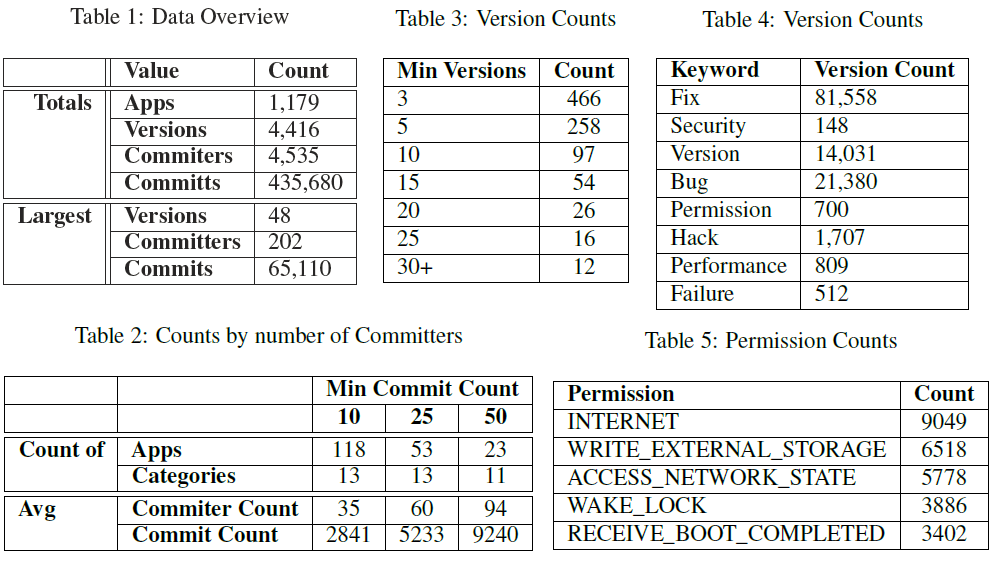
\includegraphics[width=0.98\linewidth]{./images/Tables}
%\end{figure*}

Table~\ref{table:VersionCount} displays the number of apps which have at least a specific number of versions, which is shown in the~\emph{Min Versions} column. Our dataset contains 466 apps which have at least 3 developer defined versions, and 12 apps which have 30 or more versions.


Table~\ref{table:CountsbyCommits} displays the number of apps and categories which have an average number of 10, 25, and 50 unique committers. A unique committer is defined as a commit made by someone using a unique name in the version control system for a specific app. Categories are the types of groups the app has been defined as belong to --- examples include office, internet, navigation, and games. % Figure~\ref{fig:aggregateInfo1} displays the percentage of apps in each category.


%We only take into account the number of versions for each app and do not pay any attention to the actual name of the version. For instance, it does not matter if a developer has called a version .1 or 1.0, we would only count the version number


Version control commit messages have been used in a wide range of software engineering research~\cite{bachmann2010missing} including assisting in the automatic documentation of program changes~\cite{Buse:2010:ADP:1858996.1859005} and helping with the identification of bug fixing patches~\cite{Dallmeier:2007:EBL:1321631.1321702}, which typically searches for keywords such as ``bug'' and ``fix'' in order to find bug fixing commits~\cite{Tian:2012:ILB:2337223.2337269}. For each of the 435,680 recorded commits, we have stored the author's commit message. Examples of these messages include ``Added progress bar to notification'', ``Fix a bug with the whitelist'',  and ``Fix key input in credits sequences.'' Table~\ref{table:KeywordCount} displays some keywords and the number of commits each keyword appeared in.

Information about permissions is one of the most important data-points and may be used to determine how permission settings evolve over time, which permissions are most prominently used, and if outdated permissions are still used instead of newer ones. Table~\ref{table:PermissionCounts} displays the top 5 most commonly used permissions in all AndroidManifest.xml commits along with the number of times they appeared. Complete results are available in our database for further analysis.

\subsection{Analytical Results}
%When accessing the dataset, researchers and users also have access to a wide range of analytical data.
The project website contains several reports and information pages, and users may choose to download the entire dataset. We display a wide range of aggregate information by category for all apps including the top over-permissions, most vulnerable apps according to Androrisk, and coding standards violations. As an example, Figure~\ref{fig:aggregateInfo1} illustrates the number of over-permission issues by category.

\begin{figure}[ht!]
\centering
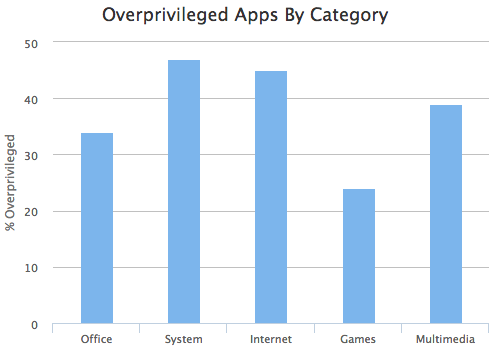
\includegraphics[width=\columnwidth, angle = 0, scale=.8]{images/Category.png}
\caption{Example Aggregate Data}
\label{fig:aggregateInfo1}
\end{figure}

Furthermore, a user can use the web portal and  search  for information about a specific app, snapshot of this search is shown in Figure~\ref{fig:appsearch}. We provide data about individual app versions as collected from static analysis including over and under permissions, Androrisk vulnerability scores, defect analysis, and code complexity. Figure~\ref{fig:specificAppInfo} shows defect information about a sample app (FBReader) over the course of multiple versions.


%Once the user selects the specific app they are searching for, the website displays information about that app including the number of versions, commits and contributors, along with various metrics about each version as collected from static analysis including over and under permissions, Androrisk vulnerability score, defect analysis, and code complexity. Figure~\ref{fig:appsearch} displays how a user may search for a specific app while Figure~\ref{fig:specificAppInfo} illustrates information about a sample app (FBReader).

\begin{figure}[ht!]
\centering
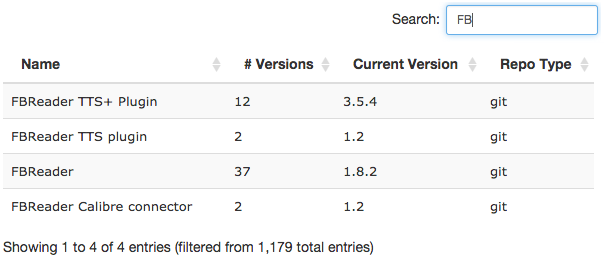
\includegraphics[width=\columnwidth, angle = 0]{images/FB_app_search.png}
\caption{App Search}
\label{fig:appsearch}
\end{figure}



\begin{figure}[ht!]
\centering
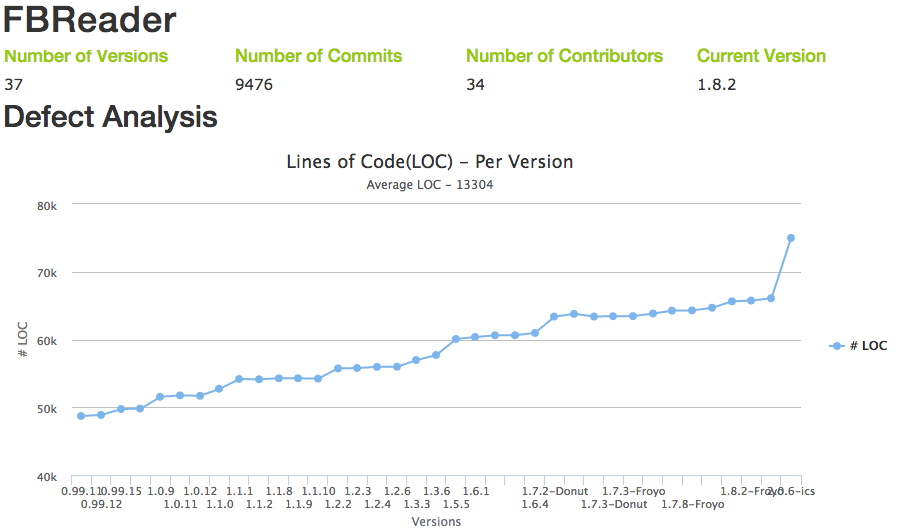
\includegraphics[width=\columnwidth, angle = 0]{images/FBReader.png}
\caption{Information About Specific App}
\label{fig:specificAppInfo}
\end{figure}


As shown in Figure~\ref{fig:webpagequery}, users may also explore the data by writing their own queries against the dataset right on the webpage.

\begin{figure}[ht!]
\centering
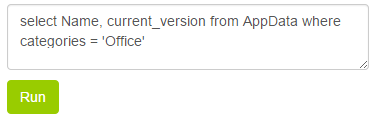
\includegraphics[width=\columnwidth, angle = 0, scale=.8]{images/webpageQuery.png}
\caption{Webpage Search Query}
\label{fig:webpagequery}
\end{figure}


\subsection{Enabled Research}

A dataset such as ours has a vast array of possible uses such as helping to better understand the development process of individual Android applications or studying dominant paradigms in app development at a more aggregate level. We next provide exemplar usage scenarios for such data.

\textbf{Facilitate research on mining software repositories}
Researchers can easily download all of the raw data as well as analytical results and conduct research experiments. An example of empirical software engineering research that could be assisted by our dataset is the exploration of the evolution of Android applications. Overall, we collected 4,416 versions of 1,179 apps, however the number of collected versions for each app widely varied. For example, 514 apps only had 1 defined version while one of the apps had 48 total versions. Future researchers may be able to use the included commit message information to study different characteristics of apps. 

Our version control history not only includes the log message, but also the committer and the time of commit, which has been previously used in wide range of mining software repositories research~\cite{Eyolfson:2011:TDD:1985441.1985464, bachmann2010missing, Buse:2010:ADP:1858996.1859005, Dallmeier:2007:EBL:1321631.1321702}.

Information collected about the AndroidManifest.xml commits can be used to determine how the app's settings and permission levels change and evolve over the time.

\textbf{Benchmark Dataset}
The collected data and the static analysis results can be used as benchmark datasets, allowing other researchers to compare their homemade static analysis results with our collected and analyzed data. This is especially useful since we are not attempting to present any specific findings or tools in our work, only data, eliminating any reason to exclude or bias information contained within the dataset.


\section{Limitations \& Future Work}
\label{sec: Limitations}

While we feel that our dataset is robust and quite useful for a variety of areas of future research, it does have some limitations and areas that will be improved upon. In the future, new static analysis tools may be added to examine the apps. Since we are storing the version control histories and source code locally, running these tools retroactively against previous versions of apps should require little effort.

% \Sam{This should be a citation, not a footnote}
While we feel that collecting more than 1,000 apps with more than 4,000 versions and over 430,000 total commits represents a substantially sized dataset, there are over 1.4 million\footnote{\url{http://www.appbrain.com/stats/number-of-android-apps}} apps available on GooglePlay, so our collection represents only a very minor portion of all apps. Additionally, we only analyzed free apps, excluding paid apps in our dataset.

Future improvements will be made to the website not only making it more usable, but also displaying the data in a more user friendly manner as well as allowing more customizable reports.


\section{Conclusion}
\label{sec: conclusion}

A dataset of Android applications with the results of the static analysis tools we have created is an important tool for understanding how Android applications are developed and maintained. The metrics we have provided are useful for understanding potential correlations between the various collected data metrics, not only for individual apps, but for apps as an aggregate as well. The collected data is publicly available on the project website: http://androsec.rit.edu

\balance
\bibliographystyle{abbrv}
\bibliography{FdroidData}

% That's all folks!
\end{document}


% ************************


%todo:
%   Example query information
%   Keywords & other info
%       Categories, General Terms, Keywords
%   Complete ER diagrams on website
%   Make sure the apks are part of the dataset as well.
%       Make sure they are mapped to specific files
%       Probably just put a link to this zip off the website 